\documentclass[12pt]{article}
%\usepackage[swedish]{babel}
%\usepackage[latin1]{inputenc}
\usepackage{graphicx}
\usepackage{fullpage}
\usepackage{pdfpages}
\usepackage{float}
\usepackage{listings}
\usepackage{color}
\title{Reprt lab 1}
\author{Group 22}
\date{\today}

\setlength{\parindent}{0pt}
\setlength{\parskip}{2ex}

\begin{document}

%\includepdf{Forsattsblad_SigSys.pdf}

\pagebreak

\maketitle

\pagebreak

\tableofcontents

\pagebreak

\section{Introduction}
This is a report for a laboration in the course Digital Signal Processing TSRT78.
The laboration consist of three assignments.
All of them are related to AR models and estimation of them.
The assignments are implemented in Matlab.
Input data for the assignments where collected by recording sounds and importing them into Matlab.
These sounds where then used to complete the assignments.

\section{Whistle}
\subsection{Task}
The first assignment is about measuring the purity of a sound compared to a sine wave. The input data is a recorded whistle and the purity is estimated using harmonic distiortion in the time and frequency domain and an AR-model of second order. The fourier transform of the whistle is shown in figure \ref{forwhis}.

\begin{figure}[H]
\centering
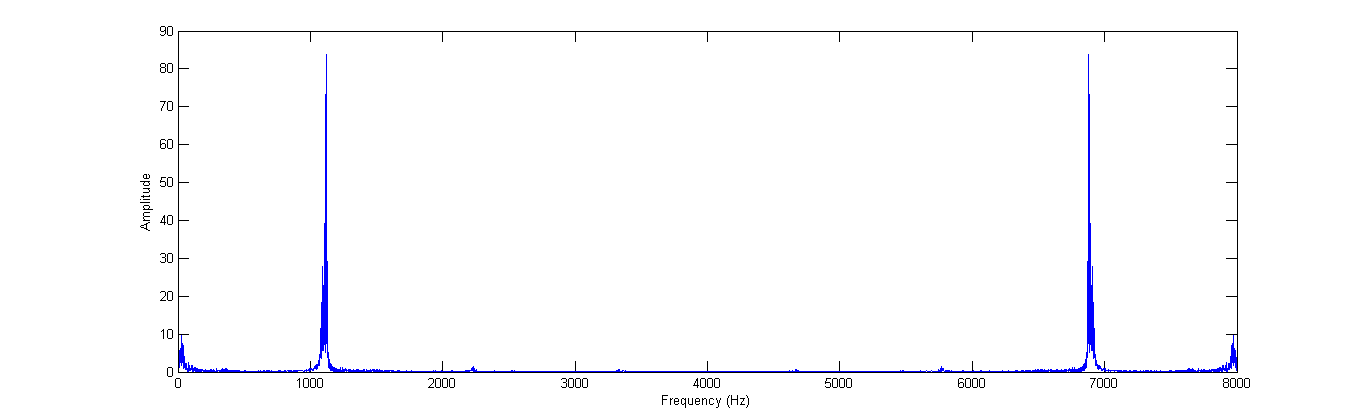
\includegraphics[width=14cm]{Fouriertranswhis.png}
\caption{The fouriertransform of the signal processed in the first assignment\label{forwhis}}
\end{figure}

\subsection{Theoretical overview}

\subsubsection{Energy and harmonic distortion}
A good way to approxiamate the purity of a periodic signal is to calculate the harmonic distorion. It is defined:

\begin{equation}Dist = 1-\frac{E_{dom. freq.}}{E_{tot.}}\end{equation}

The energy $E$ for a signal is defined as

\begin{equation}E=\int_{0}^T \vert y(t)\vert ^2 dt=\frac{1}{2\pi}\int_{\frac{-\pi}{T}}^{\frac{\pi}{T}}\vert Y(\theta)\vert ^2d\theta \end{equation}
%ssjukt fula integraler. bör fixas

where $Y(\theta)$ is the fouriertransform of $y(t)$ and T is the length of the signal. Since the signals in this laboratory are timediscrete, the energy can not be calculated this way. The integrals can instead be approximated as a sum of $N$ elements that have the width $T$, where $T$ is the length of the integration interval.

\begin{equation}
E=\int_{0}^T \vert y(t)\vert^2 dt\approx T\sum_{n=0}^{N-1}\vert y(n) \vert^2 
\label{A} 
\end{equation}

and

\begin{equation}
E=\frac{1}{2\pi}\int_{\frac{-\pi}{T}}^{\frac{\pi}{T}}\vert Y(\theta)\vert ^2d\theta \approx \frac{2\pi}{NT}\frac{1}{2\pi}\sum_{n=0}^{N-1}\vert Y(\theta) \vert^2=\frac{1}{NT}\sum_{n=0}^{N-1}\vert Y(\theta) \vert^2 
\end{equation}

\subsubsection{AR}
\label{ar} 
AR means auto-regressive and is a way of modeling signals. $AR(n)$ is defined as

\begin{equation} 
y(t)+a_1y(t-1)+...a_ny(t-n)=e(t) 
\end{equation}

where $e(t)$ is white noise. In the frequency domain

\begin{equation}
\label{Hfreq}
(1+a_1z^{-1}+..+a_nz^{-1})Y(z)=E(z) \Leftrightarrow H(z) = \frac{1}{(1+a_1z^{-1}+..+a_nz^{-1})}
\end{equation}


With the notation

\begin{equation}
(\varphi(t) =(-y(t-1) ... -y(t-n))^T,\theta = (a_1 ... a_n)^T 
\end{equation}

$y(t)$ can be defined as the linear model

\begin{equation}
y(t)=\varphi^T(t)\theta+ e(t)
\end{equation}

The optimal use of $\theta$ is

\begin{equation}
\hat{\theta}=arg_{\theta}min \frac{1}{N}\sum_{t=1}^{\infty}(y(t)-\varphi^T(t)\theta)^2
\end{equation}

which is given by

\begin{equation}
\hat{\theta}=\left(\sum_{t=1}^N\varphi(t)\varphi^T(t)\right)^{-1}\left(\sum_{t=1}^N\varphi(t)y(t)\right)
\label{enwhis}
\end{equation}

An other way of measuring purity than harmonic distortion is to use an AR-model and measure the distance to the poles from the unit circle. A pure sine-wave has its poles on the unit circle and a long distance means an unpure signal.


\subsection{Practical Execution}
The distortion of the signal can be calculated in two different ways. Either the energy of the signal is calculated in the time-domain or in the frequency domain. In this lab both methods are handeled.

The energy for the whole signal in the the time-domain is calculated according to equation \ref{A}. The energy for the dominating frequencies is acquired by filtering the signal with a bandpassfilter with the dominating frequencies in the passband. The dominating frequencies for the whistle can be approximated to 1080-1160 Hz. 

\begin{equation}
E_{tot.} \approx 0.0014, E_{dom. freq.}\approx 0.0013, Dist_{time} = 0.0511
\end{equation}

The energy for the whole signal in the frequency-domain is calculated according to equation \ref{enwhis}. The energy for the dominating frequencies can be approximated as the same sum but over only the dominating frequencies. 

\begin{equation}
E_{tot.} = \approx 
\end{equation}

% inse vad som är fel med energin och lös det!


The second order AR-model is calculated as described in section~\ref{ar}.  The AR-model of the whistle has $H(z)$ with roots $z=0.6435 \pm 0.7558i$, both with absolute value $0.9926$. That implies that the whistle is very pure. 

To verify that the AR(2) model is a good choise of estimate, the total error $\lambda$ is computed for different orders of AR-models. The results in shown in figure~\ref{whisknee}. A small error is always  a better estimate. A filter with more coefficients is on the other hand more expensive. To obtain a good but still cheap filter a "knee" is searched for in the error-function. From figure~\ref{whisknee} it is obvious that 2 is the best choice of order.   

\begin{figure}[H]
\centering
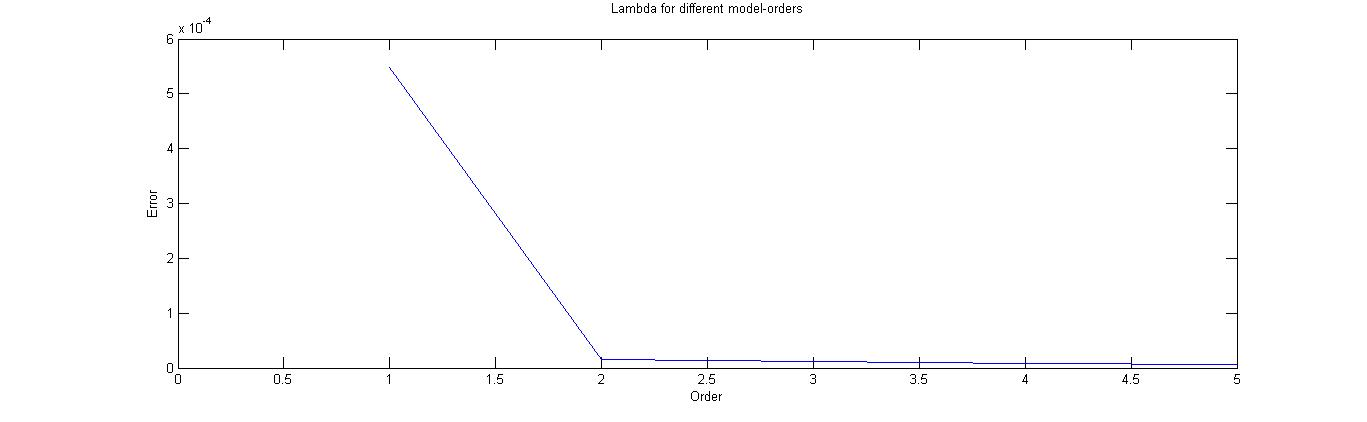
\includegraphics[width=14cm]{whistleknee.jpg}
\caption{The model-errors for different orders of AR-models.\label{whisknee}}
\end{figure}




\subsection{Results}

\section{Vowel}

\subsection{Task}
In this assignment an AR model for a the vowels 'a' and 'o' is to be estimated.
The required order of the model is unknown and to find an appropriate order is part of the assignment.
The estimated models should also be validated and different order models should be compared.

\subsection{Theoretical overview}
An AR model of the sound can be found in the same way as was done in the first assignment.
The problem this time is that a good order for the model must be found.
There are multiple ways to to do this. The 
The vowel that are estimated are voiced sounds.
This means that a pulse train is a good input signal to the model.

\subsection{Practical Execution}

\subsection{Results}

\section{Sentence}

\subsection{Task}

\subsection{Theoretical overview}

\subsection{Practical Execution}

\subsection{Results}

\section{Conclusion}



%\begin{figure}[H]
%  \centering
%  \includegraphics[width=14cm]{flow_chart.png}
%  \caption{Flow chart of Slotted ALOHA simulation.}
%\end{figure}



\clearpage
\definecolor{dkgreen}{rgb}{0,0.6,0}
\definecolor{gray}{rgb}{0.5,0.5,0.5}
\definecolor{mauve}{rgb}{0.58,0,0.82}
\lstset{
  title=\lstname,
  basicstyle=\footnotesize\ttfamily,
  keywordstyle=\color{blue},          % keyword style
  commentstyle=\color{dkgreen},       % comment style
  stringstyle=\color{mauve},         % string literal style
  showstringspaces=false,         % underline spaces within strings
}
%\lstinputlisting[language=C++]{slotted_aloha.cc}
\end{document}

